\documentclass[10pt,a4paper]{article}
\usepackage[utf8]{inputenc}
\usepackage[T1]{fontenc}
\usepackage{amsmath}
\usepackage{amssymb}
\usepackage{graphicx}

\usepackage{hyperref}
%\usepackage{url}
\usepackage{xspace}
\usepackage{float}
\restylefloat{figure}

\usepackage{rotating}
\usepackage{array}
\newcolumntype{L}{>{\centering\arraybackslash}m{4.5cm}}
\newcolumntype{I}{>{\centering\arraybackslash}m{2.5cm}}
\newcolumntype{S}{>{\centering\arraybackslash}m{1cm}}

\usepackage[table]{xcolor}    % loads also »colortbl«
\definecolor{keywordsColor}{rgb}{0.000000, 0.000000, 0.635294}
\definecolor{commentsColor}{rgb}{0.497495, 0.497587, 0.497464}
\definecolor{stringColor}{rgb}{0.558215, 0.000000, 0.135316}


\usepackage{tikz}
\usepackage{xcolor}
\definecolor{corn}{rgb}{0.98, 0.93, 0.36}
\definecolor{emerald}{rgb}{0.31, 0.78, 0.47}

\usetikzlibrary{positioning,patterns,arrows,decorations.markings,decorations.pathreplacing,shapes,shapes.misc}


\def\non{\nonumber}
\def\p{\partial}
\def\o{\over}
\def\etc{\emph{etc}.\xspace}



\title{Summary of pyVRS Non-Dimensionalization for the Semi-Spheroid Chimera Model of Embryo Swimming}
\author{Daniel Gr\"unbaum}

\begin{document}
\maketitle
This document summarizes an approach to nondimensionalizing the equations, code and parameter space underlying the semi-spheroid chimera model of embryo swimming, as implemented in pyVRS. 
One goal of this nondimensionalization is to reduce the parameter space characterizing morphology and environmental conditions. 
This facilitates understanding (and factoring out) the primary effects on swimming performance of embryo size, fluid medium density and viscosity, \etc, to simplify assessing the roles of embryo shape.
An additional goal is to derive a concise summary of performance across parameter space, and discuss morphological optimization and environmental constraints on successful embryo swimming.

The fundamental shapes in this model are chimeras constructed from two attached semi-spheroids. These semi-spheroids are matched in radius, but usually differ in height. 
We refer to a chimera of this type as a ``constitutive chimera''.

One instance of a constitutive chimera represents the surface of the embryo.
The volume inside this surface is assumed to be (mostly) tissue. 
Other constitutive chimeras may be used to approximate inclusions, containing material such as seawater or lipid (both less dense than tissue) or calcium carbonate (heavier than tissue).
If the volume of tissue is held constant, inclusions alter the volume enclosed by the surface, and typically shift the center of gravity away from the center of buoyancy.
A shift of this type results in a preferred orientation, in still water.

The ability of the embryo to swim directionally (typically upwards) depends on the relative strengths of the ``body-force'' righting moments, associated with gravity and buoyancy, compared to destabilizing environmental moments from shear and vorticity that tend to turn larvae away from their vertical orientations.
The overarching goals of the analysis are to:
\begin{enumerate}
	\item Assess how embryo size and morphology affects body-force righting moments and destabilizing environmental moments; 
	\item Assess habitats and conditions under which environmental moments exceed righting moments, compromising embryos' capacities for oriented swimming; and 
	\item Assess whether existing or hypothetical embryo sizes and morphologies are likely to encounter habitat-specific constraints, and whether observed patterns of size and morphology are consistent with predictions stemming from a requirement for oriented swimming.
\end{enumerate}
In this analysis we consider only chimeras comprising semi-spheroids.
We do not consider the more general case of semi-ellipsoids with radially asymmetrical shapes.
We also restrict our analysis to embryo shapes that are overall radially symmetrical -- that is, embryos constructed from semi-spheroids aligned along the vertical axis. 
This is in part to avoid a proliferation of parameter space, but mostly because the observed larval shapes approximate our focal class of morphologies. 
We note, though, that it is an interesting open question why early stage embryos are typically radially symmetrical\footnote{One hypothesis is that most or all such asymmetries would decrease initial stability.}. 

\section{Basic geometry of a semi-spheroid chimera}\label{GeomSect}

\begin{figure}[t] 
	\begin{center}
		\resizebox{6.5cm}{!}{
			
			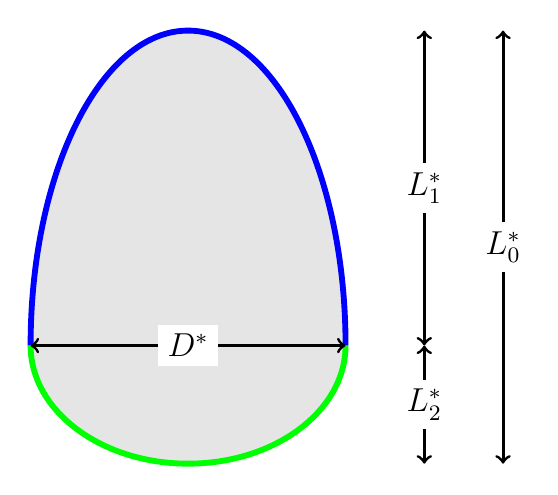
\begin{tikzpicture}
				\filldraw[blue][fill=gray!20!white,line width=0.742mm] (2,0) arc
				[
				start angle=0,
				end angle=180,
				x radius=2cm,
				y radius =4cm
				] ;
				\filldraw[green][fill=gray!20!white,line width=0.742mm] (2,0) arc
				[
				start angle=0,
				end angle=-180,
				x radius=2cm,
				y radius =1.5cm
				] ;
				\coordinate []  (A) at (-2,0)  ;
				\coordinate []  (B) at (2,0) ;
				\coordinate []  (A1) at (3,4)  ;
				\coordinate []  (B1) at (3,-1.5) ;		
				\coordinate []  (A2) at (4,4)  ;
				\coordinate []  (B2) at (4,-1.5) ;		
				\coordinate []  (equator) at (3,0) ;
				\coordinate []  (equator2) at (4,0) ;
				\path[<->] (A) edge[line width=0.371mm] node[ fill=white, anchor=center, pos=0.5,font=\bfseries] {\large $D^*$} (B);
				\path[<->] (equator) edge[line width=0.371mm] node[ fill=white, anchor=center, pos=0.5,font=\bfseries] {\large $L_1^*$} (A1);
				\path[<->] (equator) edge[line width=0.371mm] node[ fill=white, anchor=center, pos=0.5,font=\bfseries] {\large $L_2^*$} (B1);
				\path[<->] (A2) edge[line width=0.371mm] node[ fill=white, anchor=center, pos=0.5,font=\bfseries] {\large $L_0^*$} (B2);
			\end{tikzpicture}
		}
	\end{center}
	\caption{Layout of a constitutive chimera, in profile view. The view represents a vertical cross-section of a shape that is radially symmetrical about the vertical axis. The upper semi-spheroid, with diameter $D^*$ and height $L_1^*$, is shown in blue. The lower semi-spheroid, with diameter $D^*$ and height $L^*_2$, is shown in green. } \label{fig:chimera1}
\end{figure}
\noindent
Figure \ref{fig:chimera1} is a schematic showing the basic geometry of a constitutive chimera.
A constitutive chimera is parameterized by:
\begin{itemize}
	\item $D^*$, the shared diameter of its upper and lower semi-spheroids;
	\item $L_1^*$, the height of its upper semi-spheroid;
	\item $L_2^*$, the height of its  lower semi-spheroid; 
	\item $L_0^* \equiv L_1^* + L_2^*$, the total height of the chimera; and,
	\item $\alpha \equiv \frac{L_0^*}{D^*}$, an aspect ratio parameter.
\end{itemize}
We refer to the junction between the upper and lower semi-spheroids (indicated by $D$ in Figure \ref{fig:chimera1}) as the ``equator''.
The asterisks imply dimensional quantities.

From the formula for the volume of an spheroid, applied to each semi-spheroid and summed, the total volume of a constitutive chimera is
\begin{equation}\label{vol1}
	V^* = \frac{\pi}{6} {D^*}^2 \left(\frac{L_1^*+L_2^*}{2}\right) = \frac{\pi}{12} {D^*}^2 L_0^*
\end{equation} 
Equation \ref{vol1} shows that the volume is a function of diameter and total length, $L_0^*$, regardless of how that length is allocated to the upper or lower semi-spheroids.
The volume can also be expressed in terms of the aspect ratio,
\begin{equation}\label{vol2}
	V^* = \frac{\pi}{12} \alpha {D^*}^3
\end{equation} 
From a morphological perspective, this implies that an embryo of fixed height $L_0^*$ can develop into a constitutive chimera with any aspect ratio, without a change in tissue volume. 

\subsection{Embryos as composites of constitutive chimeras}

\begin{figure}[t] 
	\begin{center}
		\resizebox{6.5cm}{!}{
			
			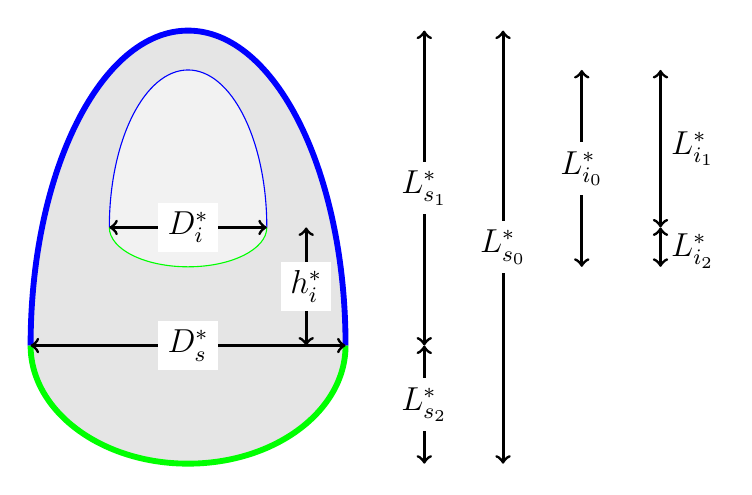
\begin{tikzpicture}
				% Outer (surface) chimera
				\filldraw[blue][fill=gray!20!white,line width=0.742mm] (2,0) arc
				[
				start angle=0,
				end angle=180,
				x radius=2cm,
				y radius =4cm
				] ;
				\filldraw[green][fill=gray!20!white,line width=0.742mm] (2,0) arc
				[
				start angle=0,
				end angle=-180,
				x radius=2cm,
				y radius =1.5cm
				] ;
				\coordinate []  (A) at (-2,0)  ;
				\coordinate []  (B) at (2,0) ;
				\coordinate []  (A1) at (3,4)  ;
				\coordinate []  (B1) at (3,-1.5) ;		
				\coordinate []  (A2) at (4,4)  ;
				\coordinate []  (B2) at (4,-1.5) ;		
				\coordinate []  (equator) at (3,0) ;
				\path[<->] (A) edge[line width=0.371mm] node[ fill=white, anchor=center, pos=0.5,font=\bfseries] {\large $D_s^*$} (B);
				\path[<->] (equator) edge[line width=0.371mm] node[ fill=white, anchor=center, pos=0.5,font=\bfseries] {\large $L_{s_1}^*$} (A1);
				\path[<->] (equator) edge[line width=0.371mm] node[ fill=white, anchor=center, pos=0.5,font=\bfseries] {\large $L_{s_2}^*$} (B1);
				\path[<->] (A2) edge[line width=0.371mm] node[ fill=white, anchor=center, pos=0.5,font=\bfseries] {\large $L_{s_0}^*$} (B2);
				\filldraw[blue][fill=gray!10!white] (1,1.5) arc
				% Inner chimera
				[
				start angle=0,
				end angle=180,
				x radius=1cm,
				y radius =2cm
				] ;
				\draw[green][fill=gray!10!white] (1,1.5) arc
				[
				start angle=0,
				end angle=-180,
				x radius=1cm,
				y radius = 0.5cm
				] ;
				\coordinate []  (A3) at (-1,1.5)  ;
				\coordinate []  (B3) at (1,1.5) ;
				\coordinate []  (A4) at (6,3.5)  ;
				\coordinate []  (B4) at (6,1) ;		
				\coordinate []  (A5) at (5,3.5)  ;
				\coordinate []  (B5) at (5,1) ;		
				\coordinate []  (equator2) at (6,1.5) ;
				\coordinate []  (h0) at (1.5,0) ;
				\coordinate []  (h1) at (1.5,1.5) ;
				\path[<->] (A3) edge[line width=0.371mm] node[ fill=white, anchor=center, pos=0.5,font=\bfseries] {\large $D_i^*$} (B3);
				\path[<->] (equator2) edge[line width=0.371mm] node[anchor=west, pos=0.5,font=\bfseries] {\large $L_{i_1}^*$} (A4);
				\path[<->] (equator2) edge[line width=0.371mm] node[anchor=west, pos=0.6,font=\bfseries] {\large $L_{i_2}^*$} (B4);
				\path[<->] (A5) edge[line width=0.371mm] node[ fill=white, anchor=center, pos=0.5,font=\bfseries] {\large $L_{i_0}^*$} (B5);
				\path[<->] (h0) edge[line width=0.371mm] node[ fill=white, anchor=center, pos=0.5,font=\bfseries] {\large $h_i^*$} (h1);
			\end{tikzpicture}
		}
	\end{center}
	\caption{Layout of a composite chimera, in profile view, with a constitutive chimera representing the exterior surface (parameterized by $D_s^*$, $L^*_{s_0}$, \etc) and a nested constitutive chimera representing an inclusion (parameterized by $D_i^*$, $L^*_{i_0}$, \etc). 
	$h_i$ is the height by which the equator of the inclusion chimera is elevated relative to the equator of the surface chimera (which may be negative). 
	%The schematic shows the inclusion chimera being co-axial with the surface chimera. 
	%In the numerical implementation, inclusions may be offset horizontally, as long as no chimera surfaces intersect.
	} \label{fig:chimera2}
\end{figure}
\noindent
Figure \ref{fig:chimera2} is a schematic showing the geometry of a composite chimera, comprising an external constitutive chimera, representing the surface of embryo tissue in contact with the fluid medium, and an internal constitutive chimera representing an inclusion such as lipid, seawater or calcium carbonate.
In the numerical model implementation, an embryo can be constructed with multiple inclusions, e.g. a ``light'' inclusion containing lipids and a ``heavy'' inclusion containing calcium carbonate.
However, to simplify calculations, the numerical model assumes there are no intersections between constitutive chimeras.
That is, \textbf{inclusion chimeras must be entirely inside the surface chimera, and entirely inside or outside of other inclusion chimeras}.

A composite chimera with one inclusion is characterized by three volumes:
\begin{itemize}
	\item $V_s^* = \frac{\pi}{12} \alpha_s {D_s^*}^3$ is the volume enclosed by the outer surface of the composite chimera, with diameter $D_s^*$ and aspect ratio $\alpha_s^*$;
	\item $V_i^* = \frac{\pi}{12} \alpha_i {D_i^*}^3$ is the volume enclosed by the inclusion constitutive chimera, with diameter $D_i^*$ and aspect ratio $\alpha_i^*$; and,
	\item $V_t^* = V_s^* - V_i^*$, the volume of tissue, which is enclosed by the outer surface but outside the inclusion. 
\end{itemize}
We can define a volume parameter, $\beta$, quantifying the factor by which total embryo volume is increased relative to tissue volume by an inclusion,
\begin{equation}\label{vol3}
	\beta = \frac{V_s^*}{V_t^*} = 1 + \frac{V_i^*}{V_t^*}.
\end{equation}
In Equation \ref{vol3}, $\beta = 1$ represents an embryo with no inclusion, $\beta = 1.5$ represents an embryo with an inclusion with volume equal to 50\% of the tissue volume, and so on.

If there are multiple inclusions, we distinguish between \textit{exposed} and \textit{contained} inclusions. 
Exposed inclusions are in contact with tissue; therefore, they displace tissue and increase volume within the embryo surface.  
If there are multiple exposed inclusions, then 
\begin{equation}\label{eqn:expincl}
	V_i^* = \sum_{j \in E} V^*_{i_j},
\end{equation}
in  Equation \ref{vol3}, where $E$ is the set of exposed inclusions.
Contained inclusions lie entirely within another inclusion; these do not displace tissue and so do not increase embryo volume.


If we assume that the embryo increases in size isometrically (that is, for a fixed aspect ratio $\alpha_s$), the change in diameter to maintain a constant tissue volume when an inclusion is added is
\begin{equation}\label{vol4}
	V_s^*  = \frac{\pi \alpha_s}{12}{D_s^*}^3 = \beta V_t^* = \frac{\pi \alpha_s \beta}{12}{D_t^*}^3,
\end{equation} 
from which 
\begin{equation}\label{vol5}
	D_s^* = \sqrt[\uproot{5}3]{\beta} D_t^*.
\end{equation}

%\begin{equation}\label{equivsphere}
%	V_{sph}^* = \frac{\pi}{6} {D_{sph}^*}^3
%\end{equation} 



\subsection{Nondimensionalization of the surface chimera}
\textbf{THIS SECTION NEEDS TO BE CHECKED!!!}

The relationships above suggest a nondimensionalization using an equivalent spherical diameter, defined as the diameter of the sphere with volume equal to that of the tissue, as a length scale:
\begin{eqnarray}\label{equivsphere}
	V_{sph}^* = \frac{\pi}{6} {D_{sph}^*}^3 = V_t^*, \non \\
	D_{sph}^* = \sqrt[\uproot{5}3]{\frac{6}{\pi} V_t^*}
\end{eqnarray} 
Equating the spherical volume to the right hand side of Equation \ref{vol2} simplifies to
\begin{equation}\label{equivD}
	D_{sph}^* = \sqrt[\uproot{5}3]{\frac{\alpha_s}{2}} ~ D_t^* = \sqrt[\uproot{5}3]{\frac{\alpha_s}{2 \beta}} ~ D_s^*
\end{equation} 
%Here, we adopt $D_s^*$ and $\alpha_s$ as notation for the equatorial diameter and aspect ratio of the surface chimera (to distinguish it from chimeras representing inclusions).
We adopt $D_{sph}^*$ as the characteristic length for nondimensionalizing embryo morphology.
For example, a nondimensionalized chimera diameter is
\begin{equation}\label{ndD}
	D_s = \frac{D_s^*}{D_{sph}^*}
\end{equation} 
where the dropped asterisk implies a nondimensional quantity.

Because $D_{sph}^*$ is defined to match volumes, this also ensures that the nondimensional volume of the tissue is equal to 1.
As a result, the body forces (excluding effects of inclusions) are also normalized to remove the primary effects of size.


From Equations \ref{equivD} and \ref{ndD},
\begin{eqnarray}\label{equivD2}
	D_t = \sqrt[\uproot{5}3]{\frac{2}{\alpha_s}}, ~ \alpha_s = \frac{2}{D_t^3}, \non \\
	D_s = \sqrt[\uproot{5}3]{\frac{2 \beta}{\alpha_s}}, ~ \alpha_s = \frac{2 \beta}{D_s^3}.
\end{eqnarray}
Equations \ref{equivD2} show that the nondimensional diameters $D_t$ and $D_s$ are fully determined by the aspect ratio $\alpha_s$ and volume parameter $\beta$, and \textit{vice versa}.


\section{Rotational movement of a sphere}\label{RotSect}
The rotation rate of a sphere of diameter $D_{sph}^*$ in a fluid of viscosity $\mu$ is 
\begin{equation}\label{rot1}
	\omega^* = \frac{T^*}{\pi \mu {D_{sph}^*}^3} = \frac{T^*}{6 \mu V_{sph}^*},	
\end{equation}
where $T^*$ is the imposed torque (i.e., the imposed moment).

We can define a rotation timescale, $\tau_{rot}^*$, as the inverse of this rate,
\begin{equation}\label{tau1}
	\tau_{rot}^* \equiv {\omega^*}^{-1} = \frac{\pi \mu {D_{sph}^*}^3}{T^*} = \frac{6 \mu V_{sph}^*}{T^*}
\end{equation}

For the timescale $\tau_{rot}^*$ to reflect the fundamental effects of size on chimera swimming, we can choose a value of $T^*$ that emerges from the equivalent sphere.
Specifically, Equation \ref{equivsphere} gives a characteristic buoyancy force of
\begin{equation}\label{charF}
	F_{sph}^* = \frac{\pi}{6} ~ \rho_{med}^* ~ g ~ {D_{sph}^*}^3 = \rho_{med}^* ~ g ~ V_{sph}^*,
\end{equation} 
where $\rho_{med}^*$ is the density of the fluid medium, and $g$ is gravitational acceleration.
Again using $D_{sph}^*$ as a characteristic length (in this case, the distance over which the characteristic force acts to generate a moment), we can assign a characteristic value to the torque:
\begin{equation}\label{charT}
	T^* = F_{sph}^* D_{sph}^* = \frac{\pi}{6} ~ \rho_{med}^* ~ g ~ {D_{sph}^*}^4 = \rho_{med}^* ~ g ~ D_{sph}^* V_{sph}^*,
\end{equation} 
This torque is an upper limit that cannot be realized (or, in most reasonable geometries, even approached).
This is because the body forces generated by inclusions will rarely approach the body force of the tissue, and the moment arm over which inclusion forces act will rarely approach the entire length of the embryo. 
Nonetheless, this torque is likely to scale in a similar way with embryo size, and the viscosity and density of the fluid medium, as torques on more realistic embryo shapes. This makes it is suitable as a characteristic value to factor out direct effects of those parameters.

Substituting this value into Equation \ref{tau1} and simplifying gives
\begin{equation}\label{tau2}
	\tau_{rot}^* = \frac{6 \mu}{\rho^*_{med} ~ g ~ D_{sph}^*}
\end{equation}
Equation \ref{tau2} reflects the fundamental proportional dependence of the rotation timescale of an equivalent sphere on size (diameter), viscosity, medium density, and gravitational acceleration.

%\subsection{Nondimensionalization of inclusion chimeras}
%This convenient fact suggests nondimensionalization based on an equivalent spherical diameter, defined as the diameter of the sphere with volume equal to that of the surface (tissue) constitutive chimera:
%\begin{equation}\label{equivsphere}
%	V_{sph}^* = \frac{\pi}{6} {D_{sph}^*}^3
%\end{equation} 
%Equating the spherical volume to the right hand side of Equation \ref{vol2} simplifies to
%\begin{equation}\label{equivD}
%	D_{sph}^* = \sqrt[\uproot{5}3]{\frac{\alpha_s}{2}} ~ D_S^*
%\end{equation} 
%Here, we adopt $D_s^*$ and $\alpha_s$ as notation for the equatorial diameter and aspect ratio of the surface chimera (to distinguish it from chimeras representing inclusions).
%
%We adopt $D_{sph}^*$ as the characteristic length for nondimensionalizing embryo morphology.
%For example, a nondimensionalized chimera diameter is
%\begin{equation}\label{ndD}
%	D_s = \frac{D_s^*}{D_{sph}^*}
%\end{equation} 
%where the dropped asterisk implies a nondimensional quantity.
%
%Because $D_{sph}^*$ is defined to match volumes, this also ensures that the nondimensional volume of the tissue is equal to 1.
%As a result, the body forces (excluding effects of inclusions) are also normalized to remove the primary effects of size.
%
%From Equations \ref{equivD} and \ref{ndD},
%\begin{eqnarray}\label{equivD2}
%	D_s = \sqrt[\uproot{5}3]{\frac{2}{\alpha_s}}, \non \\
%	\alpha_s = \frac{2}{D_s^3},
%\end{eqnarray}
%showing that the nondimensional diameter $D_s$ is fully determined by the aspect ratio $\alpha_s$, and \textit{vice versa}.


\section{Non-dimensionalized Stokes Equations}\label{NDStokesSect}
Most embryos of marine invertebrates are small enough and move slowly enough to be characterized by a very small to moderately small Reynolds Number, $Re$. 
Flows with $Re = 0$ (\textit{i.e.}, neglecting inertial effects entirely) are described by the Stokes equations, which are linear and are much easier to solve than the Navier-Stokes equations describing higher $Re$ flows.
Though the formal requirement justifying the Stokes equations is $Re \ll 1$, in practice the errors associated with using Stokes equations as approximations for flows with$Re \approx 1$ are typically small.
Here, we assume embryo swimming is characterized by the Stokes equations, accepting the small potential errors associated with inertial effects for the largest and fastest embryos to enable efficient solution techniques.

The dimensional form of the Stokes equations can be written as
\begin{eqnarray}\label{Stokes1}
	0 = \mu \left( \frac{\p^2 u^*}{\p {x^*}^2}+\frac{\p^2 u^*}{\p {y^*}^2}+\frac{\p^2 u^*}{\p {z^*}^2} \right) - \frac{\p p^*}{\p {x^*}} + f_x^*, \non \\
	0 = \mu \left( \frac{\p^2 v^*}{\p {x^*}^2}+\frac{\p^2 v^*}{\p {y^*}^2}+\frac{\p^2 v^*}{\p {z^*}^2} \right) - \frac{\p p^*}{\p {y^*}} + f_y^*, \non \\
	0 = \mu \left( \frac{\p^2 w^*}{\p {x^*}^2}+\frac{\p^2 w^*}{\p {y^*}^2}+\frac{\p^2 w^*}{\p {z^*}^2} \right) - \frac{\p p^*}{\p {z^*}} + f_z^*, \non \\
	0 =  \frac{\p u^*}{\p {x^*}}+\frac{\p v^*}{\p {y^*}}+\frac{\p w^*}{\p {z^*}} 
\end{eqnarray}
In Equations \ref{Stokes1}, the first three equations enforces conservation of momentum in the $x$, $y$ and $z$ directions in the $Re \rightarrow 0$ limit.
The last equation enforces incompressibility.

To nondimensionalize, we define nondimensional parameters $x$, $u$, $f_x$ :
\begin{itemize}
	\item $x^* = D_{sph}^* x$, $x = \frac{x^*}{D_{sph}^*}$
	\item $u^* = \frac{D_{sph}^*}{\tau_{rot}^*} u$, $u = \frac{\tau_{rot}^*}{D_{sph}^*} u^*$
	\item $f_q^* = \frac{\mu}{\tau_{rot}^* D_{sph}^*} f_q$, $f_q = \frac{\tau_{rot}^* D_{sph}^*}{\mu} f_q^*$, for each of $q = x, y, z$
	\item $p^* = \frac{\mu}{\tau_{rot}^*} p$, $p = \frac{\tau_{rot}^*}{\mu} p^*$
\end{itemize}
The scaling parameters $D_{sph}^*$ and $\tau_{rot}^*$ are as derived above in Sections \ref{GeomSect} and \ref{RotSect}.
Substituting the expression for the rotation timescale,
\begin{eqnarray}\label{NDpars}
	u = 6 \frac{\mu}{\rho^*_{med} ~ g } u^* \non \\
	f_q = \frac{D_{sph}}{\mu} 6 \frac{\mu}{\rho^*_{med} ~ g ~ D_{sph}^*} f_q^* = \frac{6}{\rho^*_{med}~  g} f_q^*, ~ q = x, y, z \non \\
	p = \frac{1}{\mu} 6 \frac{\mu}{\rho^*_{med} ~ g ~ D_{sph}^*} p^* = \frac{6}{\rho^*_{med} ~ g ~ D_{sph}^*} p^*
\end{eqnarray}
Expressing the dimensional quantities in Equations \ref{Stokes1} in terms of the nondimensional parameters in \ref{NDpars}, 
\begin{eqnarray}\label{Stokes2}
	0 = \left( \frac{\p^2 u}{\p x^2}+\frac{\p^2 u}{\p y^2}+\frac{\p^2 u}{\p z^2} \right) - \frac{\p p}{\p x} + f_x \non \\
	0 = \left( \frac{\p^2 v}{\p x^2}+\frac{\p^2 v}{\p y^2}+\frac{\p^2 v}{\p z^2} \right) - \frac{\p p}{\p y} + f_y \non \\
	0 = \left( \frac{\p^2 w}{\p x^2}+\frac{\p^2 w}{\p y^2}+\frac{\p^2 w}{\p z^2} \right) - \frac{\p p}{\p z} + f_z , \non \\
	0 =  \frac{\p u}{\p {x}}+\frac{\p v}{\p {y}}+\frac{\p w}{\p {z}}
\end{eqnarray}
Equations \ref{Stokes2} are the nondimensional form of the Stokes equations, in which space and time are rescaled such that the primary effects of embryo size, and of medium viscosity and density, are factored out.  

\section{Parameterization of the non-dimensional embryo swimming problem}\label{NDparsSect}
This section summarizes the procedure to convert dimensional parameters from a scenario of embryo swimming into their nondimensional parameter analogs, and to reconvert nondimensional results into their corresponding dimensional quantities.

The embryo parameters in the swimming embryo scenario are:
\begin{itemize}
	\item Material density, $\rho_m$, where $m$ is either tissue or an inclusion material such as seawater, lipid or calcium carbonate;
	\item Tissue volume, $V^*_t$, used to calculate $D_{sph}^*$;
	\item Surface geometry parameter (aspect ratio), $\alpha_s$ (already nondimensional);
	\item Inclusion volume, $V^*_{i_m}$ for inclusion material(s) $m$;
	\item Inclusion geometry parameter (aspect ratio), $\alpha_{i_m}$ for inclusion material(s) $m$ (already nondimensional);
	\item Inclusion offset height parameter, $h_{i_m}$ for inclusion material(s) $m$;
	\item Ciliary velocity, $v^*_{cil}$
\end{itemize}
The environmental parameters in the swimming embryo scenario are:
\begin{itemize}
	\item Fluid density, $\rho$, and viscosity, $\mu$, used with $D_{sph}^*$ to calculate $\tau_{rot}$; 
	\item Shear: $\frac{\p u^*}{\p z^*}$ and $\frac{\p w^*}{\p x^*}$; and,
	\item Time, $t^*$.
\end{itemize}


\begin{table}[h]
	\centering
	\caption{Summary of dimensional-nondimensional transformations for the swimming embryo problem. In the left column, $\sim$ is followed by the SI units of the dimensional parameter. Among dimensional-nondimensional parameter pairs, the dimensional form is labeled with an $^*$. The diameter of the equivalent sphere, $D_{sph}^*$, is given in Equation \ref{equivsphere} . The rotation timescale, $\tau^*_{rot}$, is given in Equation \ref{tau2} .} \label{tab:d2nd}
	\vspace{.25cm}
	\small
	\rowcolors{2}{gray!10}{white}
	\begin{tabular}{|I|L|lL|}
		\hline
		Dimen. param. & Conversion formula \& result & \hspace{1cm} Interpretation \\
		\hline
		$\rho_t^* \sim \mathsf{\frac{kg}{m^3}}$ & $\rho_t = \frac{1}{\rho_{med}^*} \rho_t^* $  & Density of tissue \\
		$V^*_t \sim \mathsf{m^3}$ & $V_t = \frac{1}{{D_{sph}^*}^3} V^*_t $  & Volume of tissue \\
		$\alpha_s \sim \mathsf{1}$ &    & Aspect ratio of embryo surface \\
		$\rho_m^* \sim \mathsf{\frac{kg}{m^3}}$ & $\rho_m = \frac{1}{\rho_{med}^*} \rho_m^* $  & Density of embryo material $m$ \\
		$V^*_{i_m} \sim \mathsf{m^3}$ & $V_{i_m} = \frac{1}{{D_{sph}^*}^3} V^*_{i_m} $  & Volume of inclusion $m$ \\
		$\alpha_{i_m} \sim \mathsf{1}$ &    & Aspect ratio of inclusion $m$ \\
		$h^*_{i_m} \sim \mathsf{m}$ & $h_{i_m} = \frac{1}{{D_{sph}^*}} h^*_{i_m} $  & Vertical position of inclusion $m$ \\
		$v^*_{cil} \sim \mathsf{\frac{m}{s}}$ & $v_{cil} = \frac{D_{sph}^*}{{\tau_{rot}}}  v^*_{cil}  $  & Ciliary velocity \\
		%$v^*_{cil} \sim \mathsf{\frac{m}{s}}$ & $v_{cil} = \frac{D_{sph}^*}{{\tau_{rot}}}  v^*_{cil}  = 6 \frac{\mu}{{\rho_{med}^* g}}  v^*_{cil} $  & Ciliary velocity \\
		\hline
		\vspace{0.1cm}
		$\frac{\p w^*}{\p x^*} \sim \mathsf{\frac{1}{s}}$ & $\frac{\p w}{\p x} = \tau_{rot} \frac{\p w^*}{\p x^*}  $  & Vertical shear velocity \\
		\vspace{0.1cm}
		$\frac{\p u^*}{\p z^*} \sim \mathsf{\frac{1}{s}}$ & $\frac{\p u}{\p z} = \tau_{rot} \frac{\p u^*}{\p z^*}  $  & Horizontal shear velocity \\
		\vspace{0.1cm}
		$t^* \sim \mathsf{s}$ & $t =  \frac{t^*}{\tau_{rot}}  $  & Time \\
		\hline
	\end{tabular}
\end{table}



















\end{document}